\documentclass[aspectratio=169]{beamer}

\usetheme{Boadilla}
\usefonttheme{professionalfonts}
\setbeamertemplate{navigation symbols}{}
\setbeamertemplate{itemize items}[circle]
\setbeamertemplate{enumerate items}[default]
\setbeamertemplate{headline}{}

\usepackage[utf8]{inputenc}
\usepackage[T1]{fontenc}
\usepackage{lmodern}
\usepackage{amsmath}
\usepackage{booktabs}
\usepackage{tabularx}
\usepackage{array}
\usepackage{hyperref}
\usepackage[strings]{underscore}
\usepackage{listings}
\usepackage{tikz}
\usetikzlibrary{arrows.meta,positioning,fit,calc,shapes.geometric}
\usepackage{xcolor}

\definecolor{courseblue}{HTML}{12355B}
\definecolor{coursegold}{HTML}{C98A2E}
\definecolor{courseice}{HTML}{EEF3F8}
\definecolor{coursegreen}{HTML}{2F6B4F}
\definecolor{coursegray}{HTML}{4B5563}
\definecolor{codebg}{HTML}{F7F9FC}
\definecolor{codecomment}{HTML}{5E6C84}
\definecolor{codestring}{HTML}{0B6E4F}

\setbeamercolor{palette primary}{bg=courseblue,fg=white}
\setbeamercolor{palette secondary}{bg=coursegold,fg=white}
\setbeamercolor{palette tertiary}{bg=courseblue,fg=white}
\setbeamercolor{palette quaternary}{bg=coursegold,fg=white}
\setbeamercolor{structure}{fg=courseblue}
\setbeamercolor{frametitle}{bg=courseice,fg=courseblue}
\setbeamercolor{title}{fg=courseblue}
\setbeamercolor{block title}{bg=courseblue,fg=white}
\setbeamercolor{block body}{bg=courseice,fg=black}
\setbeamercolor{normal text}{fg=black,bg=white}
\setbeamercolor{alerted text}{fg=coursegold}

\setbeamerfont{footline}{size=\scriptsize}

\setbeamertemplate{footline}{
  \leavevmode
  \hbox{
    \begin{beamercolorbox}[wd=.33\paperwidth,ht=2.8ex,dp=1.2ex,leftskip=0.8em]{palette primary}%
      University of Trieste
    \end{beamercolorbox}%
    \begin{beamercolorbox}[wd=.49\paperwidth,ht=2.8ex,dp=1.2ex,center]{palette tertiary}%
      \coursename{} \textbar{} \coursecode
    \end{beamercolorbox}%
    \begin{beamercolorbox}[wd=.18\paperwidth,ht=2.8ex,dp=1.2ex,right,rightskip=0.8em]{palette secondary}%
      \insertframenumber{} / \inserttotalframenumber
    \end{beamercolorbox}%
  }
}

\hypersetup{
  colorlinks=true,
  linkcolor=courseblue,
  urlcolor=coursegreen
}

\lstdefinestyle{coursepython}{
  language=Python,
  basicstyle=\ttfamily\footnotesize,
  keywordstyle=\color{courseblue}\bfseries,
  commentstyle=\color{codecomment}\itshape,
  stringstyle=\color{codestring},
  showstringspaces=false,
  columns=fullflexible,
  keepspaces=true,
  frame=single,
  framerule=0.6pt,
  rulecolor=\color{courseblue},
  backgroundcolor=\color{codebg},
  xleftmargin=0.4em,
  xrightmargin=0.4em,
  aboveskip=0.4em,
  belowskip=0.2em
}

\newcommand{\coursename}{Data-driven Systems Engineering}
\newcommand{\coursecode}{440MI / 305SM}
\newcommand{\coursefooter}{}

\newcommand{\learninggoals}[1]{
  \begin{block}{Learning goals}
  #1
  \end{block}
}

\newcommand{\repoactivity}[1]{
  \begin{block}{Repo activity}
  #1
  \end{block}
}

\newcommand{\readinglist}[1]{
  \begin{block}{Papers and materials}
  {\footnotesize #1}
  \end{block}
}

\newcommand{\coursecontextframe}[5]{
  \begin{frame}{Course Map and Running Cases}
  \centering
  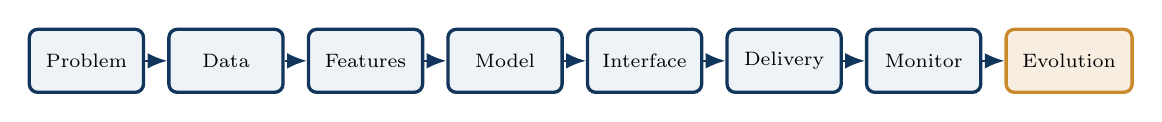
\begin{tikzpicture}[node distance=0.28cm]
  \node[flowbox, minimum width=1.45cm, minimum height=0.8cm] (problem) {\scriptsize Problem};
  \node[flowbox, minimum width=1.45cm, minimum height=0.8cm, right=of problem] (data) {\scriptsize Data};
  \node[flowbox, minimum width=1.45cm, minimum height=0.8cm, right=of data] (features) {\scriptsize Features};
  \node[flowbox, minimum width=1.45cm, minimum height=0.8cm, right=of features] (model) {\scriptsize Model};
  \node[flowbox, minimum width=1.45cm, minimum height=0.8cm, right=of model] (interface) {\scriptsize Interface};
  \node[flowbox, minimum width=1.45cm, minimum height=0.8cm, right=of interface] (delivery) {\scriptsize Delivery};
  \node[flowbox, minimum width=1.45cm, minimum height=0.8cm, right=of delivery] (monitor) {\scriptsize Monitor};
  \node[accentbox, minimum width=1.6cm, minimum height=0.8cm, right=of monitor] (evolution) {\scriptsize Evolution};
  \foreach \a/\b in {problem/data,data/features,features/model,model/interface,interface/delivery,delivery/monitor,monitor/evolution} {
    \draw[arrow] (\a) -- (\b);
  }
  \end{tikzpicture}

  \vspace{0.5em}
  \begin{block}{Today in the course}
  \textbf{Focus:} #1

  \textbf{Bridge:} #2
  \end{block}

  \begin{columns}[T]
  \column{0.48\textwidth}
  \begin{block}{Fraud case}
  {\footnotesize #3}
  \end{block}
  \column{0.48\textwidth}
  \begin{block}{Pasteurization case}
  {\footnotesize #4}
  \end{block}
  \end{columns}

  \vspace{0.3em}
  {\footnotesize \textbf{Course thread:} #5}
  \coursefooter
  \end{frame}
}

\newcommand{\classclosingframe}[4]{
  \begin{frame}{From This Class to the Next}
  \begin{block}{What stays with us}
  #1
  \end{block}

  \begin{columns}[T]
  \column{0.48\textwidth}
  \begin{block}{Project use}
  {\footnotesize #2}
  \end{block}
  \column{0.48\textwidth}
  \begin{block}{Next connection}
  {\footnotesize #3}
  \end{block}
  \end{columns}

  \vspace{0.3em}
  {\footnotesize \textbf{Course thread:} #4}
  \coursefooter
  \end{frame}
}

\tikzset{
  flowbox/.style={
    rounded corners=3pt,
    draw=courseblue,
    fill=courseice,
    very thick,
    minimum width=2.2cm,
    minimum height=0.9cm,
    align=center,
    font=\small
  },
  accentbox/.style={
    rounded corners=3pt,
    draw=coursegold,
    fill=coursegold!15,
    very thick,
    minimum width=2.2cm,
    minimum height=0.9cm,
    align=center,
    font=\small
  },
  arrow/.style={
    -{Latex[length=2.5mm,width=2mm]},
    thick,
    draw=courseblue
  }
}

\usepackage{amssymb}

\title{Class 15: Feature Engineering --- Cleaning, Curation, Selection, Construction}
\author{\coursename}
\date{}

\begin{document}

\frame{\titlepage \coursefooter}

\begin{frame}{Agenda}
\begin{itemize}
\item Why feature engineering remains necessary once every variable is numerically encoded.
\item Data cleaning: missing values, duplicates, and column-specific imputation.
\item Data curation: documenting and validating datasets for reuse.
\item Feature selection: filter, wrapper, and embedded methods.
\item Feature construction from domain knowledge, for tabular data and data streams.
\item Leakage and availability checks before deployment.
\end{itemize}
\coursefooter
\end{frame}

\begin{frame}{Why feature engineering remains necessary after encoding}
\begin{itemize}
\item Encoding (Class 14) makes a variable numerical; it does not establish whether the variable is correct, reliable, or informative.
\item Real datasets contain missing values, duplicates, and inconsistent types, which must be resolved before an encoding is meaningful.
\item Not every available variable should become a feature: some are redundant, some carry only noise, and some induce leakage.
\item Informative features are frequently absent from the raw data and must be constructed from domain knowledge.
\end{itemize}
\coursefooter
\end{frame}

\begin{frame}{Four related but distinct tasks}
\begin{tabularx}{\textwidth}{>{\bfseries}l X}
Cleaning & Treatment of missing values, duplicates, invalid values, and type errors. \\
\addlinespace[0.3em]
Curation & Organization, documentation, and validation of datasets so that they can be reused and trusted. \\
\addlinespace[0.3em]
Selection & Choice of a subset $S \subseteq \{1, \dots, d\}$ of the existing features. \\
\addlinespace[0.3em]
Construction & Definition of new features from domain logic, time, aggregation, or combinations of existing ones. \\
\bottomrule
\end{tabularx}
\coursefooter
\end{frame}

\begin{frame}{Data cleaning}
\begin{itemize}
\item Cleaning begins with an inventory of missing values, duplicates, and data types, before any modeling decision.
\item The treatment of missing values depends on the meaning of each column and on the missingness mechanism; a single global rule is rarely appropriate.
\item For categorical variables, an explicit \texttt{Unknown} category often preserves more information than imputation, since missingness itself may be informative.
\item Cleaning decisions must be documented, because they change the meaning of the data for every downstream user.
\end{itemize}
\coursefooter
\end{frame}

\begin{frame}{Cleaning example: column-specific imputation}
\begin{columns}[T]
\column{0.42\textwidth}
\centering
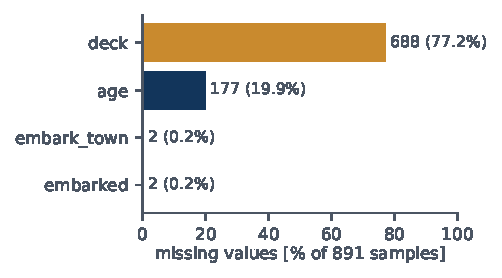
\includegraphics[width=\linewidth]{images/class15_titanic_missingness.pdf}

\vspace{0.3em}
{\scriptsize Titanic data used in \texttt{notebooks/Class4\_DataEngineering.ipynb}, $n = 891$.\par}
\column{0.56\textwidth}
\begingroup\footnotesize
\begin{tabularx}{\linewidth}{>{\ttfamily}l >{\raggedright\arraybackslash}p{1.7cm} >{\raggedright\arraybackslash}X}
\normalfont\bfseries Column & \bfseries Policy & \bfseries Rationale \\
\toprule
deck & explicit \texttt{Unknown} & 77\% missing: imputation would invent most values; missingness may be informative \\
\addlinespace[0.3em]
age & median (28.0) & numerical, moderate missingness; the median is robust to outliers \\
\addlinespace[0.3em]
embarked & mode (\texttt{S}) & two missing values: negligible effect \\
\addlinespace[0.3em]
embark\_town & explicit \texttt{Unknown} & duplicates \texttt{embarked} (see the $\chi^2$ ranking) \\
\bottomrule
\end{tabularx}
\par\endgroup
\vspace{0.4em}
{\footnotesize The dataset also contains 107 duplicated rows; without a passenger identifier, they cannot be distinguished from distinct passengers with identical attributes, so they were kept.\par}
\end{columns}
\coursefooter
\end{frame}

\begin{frame}{Data curation}
\begin{itemize}
\item Curation makes a cleaned dataset reusable by analysts other than those who cleaned it.
\item A data dictionary records the meaning, unit, and valid range of every column.
\item Dataset versioning, or at least a recorded extraction date, allows later experiments to be compared on equal terms.
\item Validation rules (schema and range checks) detect upstream problems before they reach the modeling stage.
\end{itemize}
\begin{block}{Repository example}
The specification of the fraud case in \texttt{documents/FraudDetectionAsaService.pdf} acts as a curated data description: it documents the dataset and the workflow explicitly instead of leaving them implicit in a notebook.
\end{block}
\coursefooter
\end{frame}

\begin{frame}{Curation example: a data dictionary for the pasteurization sensors}
\begingroup\footnotesize
\renewcommand{\arraystretch}{1.2}
\begin{tabularx}{\textwidth}{>{\ttfamily}l l >{\raggedright\arraybackslash}X l l}
\normalfont\bfseries Variable & \bfseries Unit & \bfseries Meaning & \bfseries Observed range & \bfseries Validation rule \\
\toprule
T & °C & Product temperature; set point 72 during Hold & 3.95 -- 72.24 & $0 \le T \le 80$ \\
pH & --- & Acidity of the milk & 6.60 -- 6.69 & $6.4 \le \mathrm{pH} \le 6.9$ \\
Kappa & mS/cm & Electrical conductivity & 2.91 -- 5.27 & $\kappa > 0$ \\
Mu & cP & Viscosity; decreases with temperature & 1.42 -- 2.45 & $\eta > 0$ \\
Tau & relative & Turbidity & 0.14 -- 1.17 & $\tau \ge 0$ \\
Q\_in, Q\_out & n.s. & Inflow and outflow; 1.5 when active, 0 otherwise & 0.00 -- 1.70 & $Q \ge 0$ \\
P & n.s. & Pressure & 0.81 -- 1.62 & $P > 0$ \\
dTdt & °C/s & Derived: $(T_t - T_{t-1})/\Delta t$ & $-5.48$ -- $3.61$ & --- \\
\bottomrule
\end{tabularx}
\par\endgroup
\vspace{0.4em}
{\scriptsize Observed ranges over 100 batches simulated with \texttt{synth\_sensors.py}; n.s.: unit not specified in the simulator; validation rules are proposed examples. Such a table, versioned with the data, is the core of a datasheet for the dataset.\par}
\coursefooter
\end{frame}

\begin{frame}{Feature selection: filter, wrapper, embedded}
\begingroup\small
Given $d$ candidate features, selection seeks a subset $S \subseteq \{1, \dots, d\}$ that maximizes a criterion $J(S)$. The three families differ in how $J$ is defined.
\par\endgroup
\vspace{0.5em}
\begin{tabularx}{\textwidth}{>{\bfseries}l X}
Filter & $J$ is a model-independent statistic computed for each feature, e.g.\ correlation, mutual information, or the $\chi^2$ statistic. \\
\addlinespace[0.3em]
Wrapper & $J(S)$ is the validation performance of a model trained on $S$; subsets are explored by a search strategy (e.g.\ forward or backward selection). \\
\addlinespace[0.3em]
Embedded & Selection occurs during training, e.g.\ the least absolute shrinkage and selection operator (Lasso), $\min_{\boldsymbol\beta} \|\mathbf{y} - X\boldsymbol\beta\|_2^2 + \lambda\|\boldsymbol\beta\|_1$, which sets some coefficients exactly to zero. \\
\bottomrule
\end{tabularx}
\coursefooter
\end{frame}

\begin{frame}{Filter example: the $\chi^2$ test of independence}
\begin{columns}[T]
\column{0.44\textwidth}
\begingroup\small
Observed counts $O$ (expected $E$ under independence), \texttt{sex} $\times$ \texttt{survived}:
\par\endgroup
\vspace{0.4em}
\centering
\begingroup\footnotesize
\begin{tabular}{l c c c}
& died & survived & total \\
\toprule
female & 81 \textcolor{coursegray}{(193.5)} & 233 \textcolor{coursegray}{(120.5)} & 314 \\
male & 468 \textcolor{coursegray}{(355.5)} & 109 \textcolor{coursegray}{(221.5)} & 577 \\
\midrule
total & 549 & 342 & 891 \\
\bottomrule
\end{tabular}
\par\endgroup
\vspace{0.6em}
\[
\chi^2 = \sum_{\text{cells}} \frac{(O - E)^2}{E} = 263.1
\]
\vspace{-0.4em}
{\footnotesize with $E = (\text{row total} \times \text{column total})/n$.\par}
\column{0.54\textwidth}
\begin{itemize}\footnotesize
\item If \texttt{sex} and \texttt{survived} were independent, each cell would contain approximately its expected count $E$.
\item The larger $\chi^2$, the further the observed table is from independence, i.e.\ the stronger the association with the target ($p < 10^{-58}$ here, with 1 degree of freedom).
\item It is a filter criterion: computed per feature, before and independently of any model.
\item \textbf{Caution:} \texttt{sklearn.feature\_selection.chi2} treats feature values as non-negative counts. Applied to label-encoded nominal variables, it does not compute this test, and its score depends on the arbitrary codes (92.7 instead of 263.1 for \texttt{sex}).
\end{itemize}
\end{columns}
\coursefooter
\end{frame}

\begin{frame}{Filter result: $\chi^2$ ranking of categorical features}
\begin{columns}[T]
\column{0.52\textwidth}
\centering
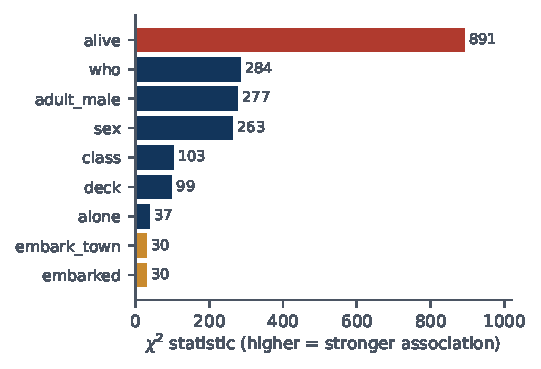
\includegraphics[width=\linewidth]{images/class15_titanic_chi2.pdf}
\column{0.46\textwidth}
\begin{itemize}\footnotesize
\item \textbf{\textcolor[HTML]{B03A2E}{alive}} attains the maximum $\chi^2 = n = 891$: it restates the target (\texttt{yes}/\texttt{no}). A filter ranks a leaking feature first; it must be removed by inspection, not by score.
\item \textbf{\textcolor{coursegold}{embarked}} and \textbf{\textcolor{coursegold}{embark\_town}} have identical scores: they encode the same information, so one of them is redundant.
\item \texttt{who}, \texttt{adult\_male}, and \texttt{sex} rank high together because they overlap strongly; a univariate filter cannot detect this redundancy.
\end{itemize}
\end{columns}
\vspace{0.3em}
{\scriptsize $\chi^2$ test of independence on the contingency table of each feature with \texttt{survived}; missing values treated as an explicit category.\par}
\coursefooter
\end{frame}

\begin{frame}{Selection example: is \texttt{is\_alone} redundant?}
\centering
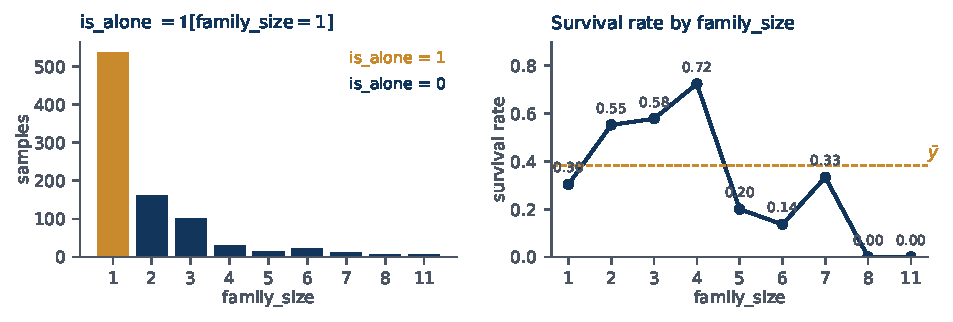
\includegraphics[width=0.92\textwidth,height=0.42\textheight,keepaspectratio]{images/class15_titanic_family_size.pdf}

\vspace{0.2em}
\begin{itemize}\footnotesize
\item \textbf{Informationally redundant:} \texttt{is\_alone} is a deterministic function of \texttt{family\_size}; it adds no information, which would justify removing it.
\item \textbf{Not redundant for a linear model:} survival is non-monotonic in \texttt{family\_size}, so its linear correlation with \texttt{survived} is only $0.02$, whereas that of \texttt{is\_alone} is $-0.20$. The indicator acts as a non-linear transformation that a linear model cannot build by itself.
\item Redundancy is therefore relative to the model family: a decision tree can recover \texttt{is\_alone} with a single split; logistic regression cannot. The notebook keeps it, and the test accuracy of its logistic regression rises from 0.804 to 0.810 (one additional correct prediction out of 179).
\end{itemize}
\coursefooter
\end{frame}

\begin{frame}{Feature construction from domain knowledge}
\begin{itemize}
\item Informative features usually originate from an understanding of the problem rather than from generic mathematical transformations.
\item Aggregations (counts, sums), ratios, and simple domain rules often outperform automated feature generation.
\item Each constructed feature should be checked for redundancy with the variables from which it was derived.
\item The rationale for every constructed feature should be stated explicitly, in one sentence.
\end{itemize}
\coursefooter
\end{frame}

\begin{frame}{Construction example: domain rules}
\begingroup\footnotesize
\renewcommand{\arraystretch}{1.3}
\begin{tabularx}{\textwidth}{>{\ttfamily}l >{\raggedright\arraybackslash}p{4.2cm} l >{\raggedright\arraybackslash}X}
\normalfont\bfseries Feature & \bfseries Definition & \bfseries Scale & \bfseries Rationale \\
\toprule
family\_size & $\texttt{sibsp} + \texttt{parch} + 1$ & ratio & Passengers travelling together share their fate; survival rate rises from 0.30 (alone) to 0.72 (four members), then falls \\
is\_alone & $\mathbf{1}[\texttt{family\_size} = 1]$ & binary & Isolates the largest and least favoured group (537 passengers) \\
title & \texttt{man}$\to$Mr, \texttt{woman}$\to$Mrs, \texttt{child}$\to$Master & nominal & One-to-one relabelling of \texttt{who}: adds no information (identical $\chi^2$) \\
\bottomrule
\end{tabularx}
\par\endgroup
\vspace{0.6em}
\begin{itemize}\footnotesize
\item From \texttt{notebooks/Class4\_DataEngineering.ipynb}: each constructed feature is a short, explainable rule. A useful construction combines or transforms information; a bijective relabelling, such as \texttt{title}, only renames it.
\item In the fraud case, behavioural features (rolling transaction count, deviation from recent spending) would require a card identifier, which the anonymized dataset does not provide.
\end{itemize}
\coursefooter
\end{frame}

\begin{frame}{Feature construction for streams and sensors}
\begin{columns}[T]
\column{0.5\textwidth}
\centering
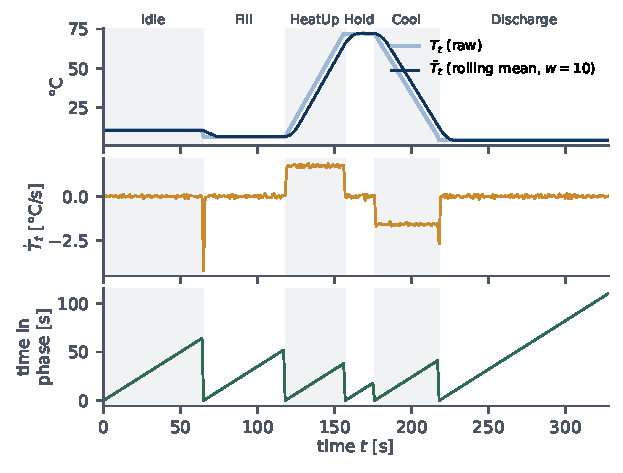
\includegraphics[width=\linewidth]{images/class15_stream_features.pdf}

{\tiny One batch generated by \texttt{pasteurization/synth\_sensors.py}.\par}
\column{0.48\textwidth}
\begingroup\footnotesize
Features computed from the raw temperature $T_t$:
\begin{itemize}
\item \textbf{Rolling mean:} $\bar{T}_t = \frac{1}{w}\sum_{i=0}^{w-1} T_{t-i}$; smooths noise and indicates stability, at the cost of a lag of about $w/2$ samples.
\item \textbf{Rate of change:} $\dot{T}_t = (T_t - T_{t-1})/\Delta t$; separates HeatUp ($> 0$) from Cool ($< 0$), which the raw value cannot.
\item \textbf{Time in phase:} seconds since the last change of state; a state-aware feature that distinguishes a slow heating from a normal one.
\end{itemize}
All three use only past observations, so they can be computed online, one sample at a time, exactly as in production.
\par\endgroup
\end{columns}
\coursefooter
\end{frame}

\begin{frame}{Engineered features change the dependence structure}
\begin{columns}[T]
\column{0.55\textwidth}
\centering
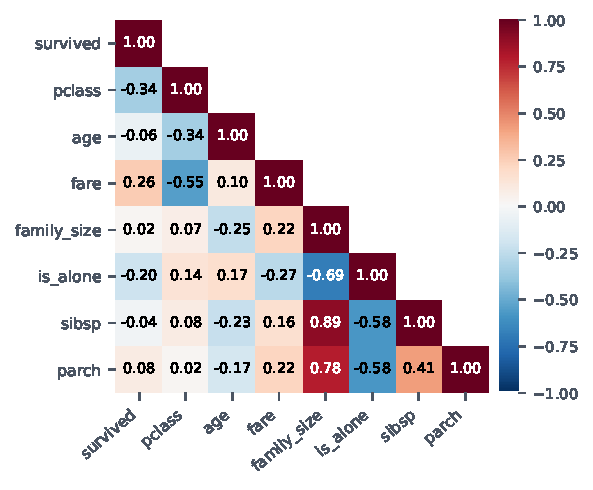
\includegraphics[width=\linewidth]{images/class15_titanic_correlation.pdf}
\column{0.43\textwidth}
\begin{itemize}\footnotesize
\item Pearson correlations after cleaning (\texttt{age} imputed with the median).
\item \texttt{family\_size} is strongly correlated with its components \texttt{sibsp} ($0.89$) and \texttt{parch} ($0.78$): keeping all three adds collinearity without new information.
\item \texttt{is\_alone} has a larger linear association with \texttt{survived} ($-0.20$) than \texttt{family\_size} ($0.02$), as discussed in the selection example.
\item Pearson correlation measures only linear dependence; a near-zero value does not imply that a feature is uninformative.
\end{itemize}
\end{columns}
\coursefooter
\end{frame}

\begin{frame}{Leakage and availability checks}
\begin{itemize}
\item Is the feature available at prediction time, or does it use information from the future?
\item Does it encode a post-decision outcome, such as the result of a manual review?
\item Is it computed identically in production and in the notebook?
\item Does it depend on joins or upstream systems that may be unavailable at inference time?
\end{itemize}
\vspace{0.3em}
{\footnotesize The complete taxonomy of leakage (target, preprocessing, temporal, group, duplicate, model selection) was presented in Class 13.}
\coursefooter
\end{frame}

\begin{frame}{Repository connections}
\repoactivity{
\begin{itemize}
\item \texttt{notebooks/Class4\_DataEngineering.ipynb} covers cleaning, $\chi^2$ selection, and domain-driven construction end to end.
\item \texttt{pasteurization/synth\_sensors.py} provides the constructed feature for time series data (\texttt{dTdt}).
\item \texttt{streamlit/modeling.py} saves the fitted scaler together with the model, illustrating that preprocessing decisions must be persisted with the model rather than applied once in a notebook.
\end{itemize}
}
\coursefooter
\end{frame}

\begin{frame}{Papers and materials}
\readinglist{
\fontsize{6.8}{8.2}\selectfont
\begin{columns}[T]
\column{0.5\textwidth}
\begin{itemize}\setlength{\itemsep}{1pt}
\item Guyon, I., Elisseeff, A. (2003). An introduction to variable and feature selection. \emph{Journal of Machine Learning Research}, 3, 1157--1182.
\item Kohavi, R., John, G.\,H. (1997). Wrappers for feature subset selection. \emph{Artificial Intelligence}, 97(1--2), 273--324.
\item Tibshirani, R. (1996). Regression shrinkage and selection via the lasso. \emph{Journal of the Royal Statistical Society: Series B}, 58(1), 267--288.
\item Little, R.\,J.\,A., Rubin, D.\,B. (2019). \emph{Statistical Analysis with Missing Data}, 3rd ed. Wiley.
\end{itemize}
\column{0.5\textwidth}
\begin{itemize}\setlength{\itemsep}{1pt}
\item Gebru, T., Morgenstern, J., Vecchione, B., Wortman Vaughan, J., Wallach, H., Daum\'e III, H., Crawford, K. (2021). Datasheets for datasets. \emph{Communications of the ACM}, 64(12), 86--92.
\item Domingos, P. (2012). A few useful things to know about machine learning. \emph{Communications of the ACM}, 55(10), 78--87.
\item Zheng, A., Casari, A. (2018). \emph{Feature Engineering for Machine Learning}. O'Reilly.
\item scikit-learn User Guide: \href{https://scikit-learn.org/stable/modules/feature_selection.html}{feature selection}; \href{https://scikit-learn.org/stable/modules/compose.html}{pipelines and composite estimators}.
\end{itemize}
\end{columns}
}
\coursefooter
\end{frame}

\begin{frame}{Take-away message}
\vfill
\centering
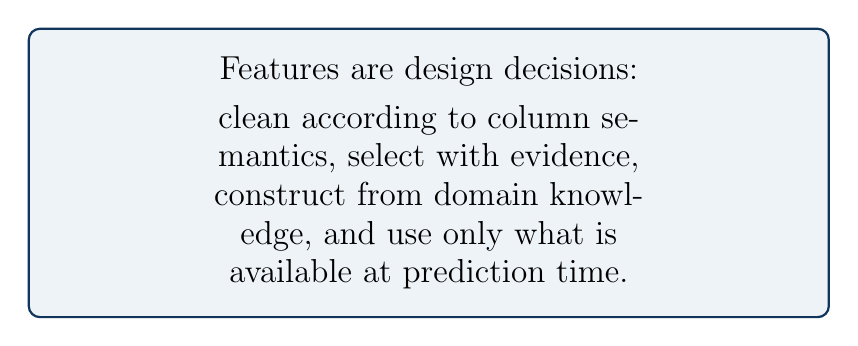
\begin{tikzpicture}
\node[fill=courseice, draw=courseblue, thick, rounded corners=4pt, inner sep=10pt, text width=0.78\textwidth, align=center, font=\large] {Features are design decisions:\\[0.3em] clean according to column semantics, select with evidence,\\ construct from domain knowledge, and use only what is\\ available at prediction time.};
\end{tikzpicture}

\vfill
{\Large\bfseries\color{courseblue} Thank you for your attention.}

\vspace{0.4em}
{\small\color{coursegray} Next: Class 16 --- machine learning modeling, experiment tracking, evaluation, and decision-making.}
\vfill
\coursefooter
\end{frame}

\end{document}
